\documentclass[ignorenonframetext,]{beamer}
\setbeamertemplate{caption}[numbered]
\setbeamertemplate{caption label separator}{: }
\setbeamercolor{caption name}{fg=normal text.fg}
\beamertemplatenavigationsymbolsempty
\usepackage{lmodern}
\usepackage{amssymb,amsmath}
\usepackage{ifxetex,ifluatex}
\usepackage{fixltx2e} % provides \textsubscript
\ifnum 0\ifxetex 1\fi\ifluatex 1\fi=0 % if pdftex
  \usepackage[T1]{fontenc}
  \usepackage[utf8]{inputenc}
\else % if luatex or xelatex
  \ifxetex
    \usepackage{mathspec}
  \else
    \usepackage{fontspec}
  \fi
  \defaultfontfeatures{Ligatures=TeX,Scale=MatchLowercase}
\fi
% use upquote if available, for straight quotes in verbatim environments
\IfFileExists{upquote.sty}{\usepackage{upquote}}{}
% use microtype if available
\IfFileExists{microtype.sty}{%
\usepackage{microtype}
\UseMicrotypeSet[protrusion]{basicmath} % disable protrusion for tt fonts
}{}
\newif\ifbibliography
\hypersetup{
            pdfborder={0 0 0},
            breaklinks=true}
\usepackage{longtable,booktabs}
\usepackage{caption}
% These lines are needed to make table captions work with longtable:
\makeatletter
\def\fnum@table{\tablename~\thetable}
\makeatother
\usepackage{graphicx,grffile}
\makeatletter
\def\maxwidth{\ifdim\Gin@nat@width>\linewidth\linewidth\else\Gin@nat@width\fi}
\def\maxheight{\ifdim\Gin@nat@height>\textheight0.8\textheight\else\Gin@nat@height\fi}
\makeatother
% Scale images if necessary, so that they will not overflow the page
% margins by default, and it is still possible to overwrite the defaults
% using explicit options in \includegraphics[width, height, ...]{}
\setkeys{Gin}{width=\maxwidth,height=\maxheight,keepaspectratio}

% Prevent slide breaks in the middle of a paragraph:
\widowpenalties 1 10000
\raggedbottom

\AtBeginPart{
  \let\insertpartnumber\relax
  \let\partname\relax
  \frame{\partpage}
}
\AtBeginSection{
  \ifbibliography
  \else
    \let\insertsectionnumber\relax
    \let\sectionname\relax
    \frame{\sectionpage}
  \fi
}
\AtBeginSubsection{
  \let\insertsubsectionnumber\relax
  \let\subsectionname\relax
  \frame{\subsectionpage}
}

\setlength{\parindent}{0pt}
\setlength{\parskip}{6pt plus 2pt minus 1pt}
\setlength{\emergencystretch}{3em}  % prevent overfull lines
\providecommand{\tightlist}{%
  \setlength{\itemsep}{0pt}\setlength{\parskip}{0pt}}
\setcounter{secnumdepth}{0}
\usepackage[british]{babel}
\usepackage{graphicx,hyperref,anderson,url,booktabs,dcolumn,ragged2e}
\usepackage{fontawesome}

\title[Regression models]{Regression models for epidemiological research}
\subtitle{Advanced Epidemiology}
\date{April 18, 2017}

\author[Brooke Anderson]{
  Brooke Anderson \\\medskip
  {\small \faEnvelope: \url{brooke.anderson@colostate.edu}} \\
  {\small \faGithub:  \url{www.github.com/geanders}}}

\institute[Colorado State University]{
  Department of Environmental \& Radiological Health Sciences \\
  Environmental Epidemiology Section \\
  Colorado State University}

\date{}

\begin{document}

\begin{frame}
  \titlepage
\end{frame}

\begin{frame}{Further reading and sources}

\begin{itemize}
\tightlist
\item
  Woodward (2014) \emph{Epidemiology: Study Design and Data Analysis.}
  Chapman \& Hall.
\item
  Vittinghoff et al. (2005) \emph{Regression Methods in Biostatistics:
  Linear, Logistic, Survival, and Repeated Measures Models.} Springer.
\item
  Harrell. (2001) \emph{Regression Modelling Strategies: With
  Applications to Linear Models, Logistic and Ordinal Regression, and
  Survival Analysis.} Springer.
\end{itemize}

\end{frame}

\begin{frame}{Basics of logarithms}

There are a few basics of logartithms you should keep in mind for this
lecture (these all use \(log\) for a natural logarithm):

\begin{enumerate}
\def\labelenumi{\arabic{enumi}.}
\tightlist
\item
  If \(log(a) = b\), then \(a = e^b\).
\item
  \(log(e^a) = a\). Similarly, \(e^{log(a)} = a\).
\item
  \(log(1) = 0\) and \(e^0 = 1\).
\item
  \(log(a * b) = log(a) + log(b)\).
\item
  \(log(a / b) = log(a) - log(b)\). As a result, \(log(1/a) = -log(a)\).
\end{enumerate}

\end{frame}

\begin{frame}{General model equation for generalized linear regression}

Systematic part of generalized linear models (GLMs):

\[ 
g(E[Y_i]) = \beta_0 + \beta_1X_1 + \beta_2X_2 + \beta_3X_3 + ...
\] where:

\begin{itemize}
\tightlist
\item
  \(E[Y_i]\) is the expected value of the outcome (\(Y_i\)) for
  observation \(i\)
\item
  \(g(.)\) is a function linking the expected value of the outcomes to
  the predictors (identity function for linear regression, logit
  function for logistic regression, etc.)
\item
  \(\beta_0\) is the model intercept
\item
  \(X_1\), \(X_2\), \(X_3\), etc., are predictor variables
\item
  \(\beta_1\), \(\beta_2\), \(\beta_3\), etc., are parameters describing
  the relationship between the predictor variables and the outcome
\end{itemize}

The right-hand side of this model equation is the \textbf{linear
predictor}.

\end{frame}

\begin{frame}{General model equation for generalized linear regression}

Random part of GLMs:

\begin{itemize}
\tightlist
\item
  What is the distribution of the outcome (\(Y_i\)) conditional on the
  observed values of the predictors (\(X_1\), \(X_2\), etc.)?
\end{itemize}

\begin{block}{Fitting GLMs}
GLMs are fit through \textbf{maximum-likelihood estimation}. For each candidate model, the \textbf{likelihood} of the data (joint probability of the data) under that model is measured. The \textbf{maximum-likelihood estimates} for the parameters are the values that maximize the likelihood of the observed data. 
\end{block}

\end{frame}

\begin{frame}{General model equation for generalized linear regression}

\begin{block}{Simple regression}
If only one explanatory variable is included, it's a "simple" regression: 
\begin{equation*} 
g(E[Y_i]) = \beta_0 + \beta_1X_1 
\end{equation*}
\end{block}

\begin{block}{Multiple regression}
If two or more explanatory variables are included, it's a "multiple" regression: 
\begin{equation*}
g(E[Y_i]) = \beta_0 + \beta_1X_1 + \beta_2X_2 + \beta_3X_3 + ...
\end{equation*}
\end{block}

\end{frame}

\begin{frame}{An epidemiologist walks into a movie theater\ldots{}}

\begin{columns}
\begin{column}{0.45\textwidth}
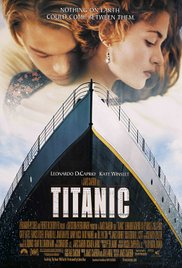
\includegraphics[width=\textwidth]{images/titanic_poster.jpg}
\end{column}
\begin{column}{0.55\textwidth}
The mortality outcomes, by sex, of passengers on the Titanic were (note: some passengers with missing data have been excluded):\\[0.5ex]

\centering

\begin{tabular}{llD{.}{.}{0}D{.}{.}{0}}
\toprule
 && \multicolumn{2}{c}{Outcome}\\
\cmidrule{3-3}\cmidrule{4-4}
Sex && \multicolumn{1}{c}{Survived}&\multicolumn{1}{c}{Died}\\
\midrule
Female && 292 & 96 \\
Male   && 135 & 523\\
\bottomrule
\end{tabular}

\medskip

\justifying

\footnotesize{Data obtained from \url{http://biostat.mc.vanderbilt.edu/wiki/Main/DataSets}. Original data source: Hind (1999) \textit{Encyclopedia Titanica.} \url{http://atschool.eduweb.co.uk/phind}. Figure source: \url{http://www.imdb.com}}
\end{column}
\end{columns}

\end{frame}

\begin{frame}{Example-- Surviving the Titanic}

Based on this table (i.e., using contingency table methods), determine
and discuss:

\begin{itemize}
\tightlist
\item
  Does sex affect the odds of dying during the Titanic sinking?
\item
  Are the odds that someone like Jack will die on the Titanic versus the
  odds that someone like Rose will?
\item
  How do these two questions differ?
\item
  Are the odds of dying on the Titanic significantly higher
  (statistically) for males versus females? What about for someone like
  Jack versus someone like Rose?
\item
  What other information would you like to have to better answer these
  questions? How would the information help to answer the previous
  questions?
\end{itemize}

\end{frame}

\begin{frame}{Example-- Surviving the Titanic}

\centering

\begin{tabular}{llD{.}{.}{0}D{.}{.}{0}}
\toprule
 && \multicolumn{2}{c}{Outcome}\\
\cmidrule{3-3}\cmidrule{4-4}
Sex && \multicolumn{1}{c}{Survived}&\multicolumn{1}{c}{Died}\\
\midrule
Female && 292 & 96 \\
Male   && 135 & 523\\
\bottomrule
\end{tabular}

\begin{itemize}
\tightlist
\item
  The odds for dying on the Titanic for females is
  \(\frac{96}{292} = 0.33\)
\item
  The odds for dying on the Titanic for males is
  \(\frac{523}{135} = 3.87\)
\item
  The odds ratio for dying on the Titanic for males compared to females
  is \(\frac{523 * 292}{135 * 96} = 11.78\)
\item
  The log odds ratio is \(log(11.78) = 2.47\)
\item
  The estimated standard error for the log odds ratio is
  \(\sqrt{\frac{1}{292} + \frac{1}{96} + \frac{1}{135} + \frac{1}{523}} = 0.15\)
\item
  The 95\% confidence interval for the odds ratio is (8.74, 15.88)
\end{itemize}

\end{frame}

\begin{frame}{Logistic function}

Logistic function, with \(p_i = Pr(Y_i = 1 | X_i)\):

\[
p_i = \frac{1}{1 + e^{-\beta_0-\beta_1X_i}}
\]

Plot of logistic function with \(\beta_0\) = 0, \(\beta_1\) = 1 (note
that y is always between 0 and 1):

\begin{center}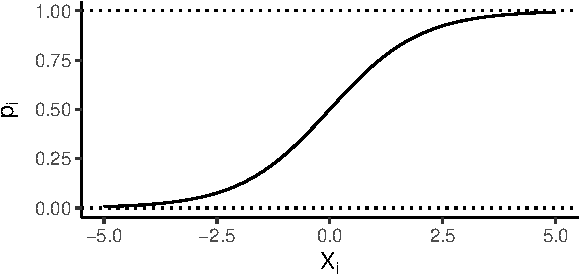
\includegraphics[width=3in]{regression_files/figure-beamer/unnamed-chunk-4-1} \end{center}

\end{frame}

\begin{frame}{Logit function}

Notice what happens if you change the equation so the right-hand side
matches the typical model equation format for a GLM. \medskip

Before:

\[
p_i = \frac{1}{1 + e^{-\beta_0 - \beta_1X_i}}
\]

After:

\[
log(\frac{p_i}{1 - p_i}) = \beta_0 + \beta_1X_i
\]

\medskip The left-hand side of this equation is the \textbf{logit} of
\(p_i\).

\end{frame}

\begin{frame}{Logistic regression example}

Let's fit a logistic regression for the previous example on sex and risk
of dying in the Titanic sinking. The systematic part of this model is:

\[
log(\frac{p_i}{1 - p_i}) = \beta_0 + \beta_1X_{1,i}
\]

where:

\begin{itemize}
\tightlist
\item
  \(p_i\): Probability person \(i\) died during the sinking,
  \(Pr(Y_i = 1 | X_i)\)
\item
  \(Y_i\): Whether person \(i\) died during the sinking
\end{itemize}

\begin{equation*}
    X_i=
    \begin{cases}
      0 \text{ if person \textit{i} is female} \\
      1 \text{ if person \textit{i} is male}
    \end{cases}
\end{equation*}

The random part of the model is: Outcomes (\(Y_i\)) follow a binomial
distribution.

\end{frame}

\begin{frame}{Interpreting coefficients-- logistic regression}

For males, this equation evaluates to:

\[
log(\frac{p_m}{1 - p_m}) = \beta_0 + \beta_1*1 = \beta_0 + \beta_1
\]

For females, this equation evaluates to:

\[
log(\frac{p_f}{1 - p_f}) = \beta_0 + \beta_1*0 = \beta_0 
\]

Therefore:

\begin{itemize}
\tightlist
\item
  The log odds for males is estimated by \(\beta_0 + \beta_1\)
\item
  The log odds for females is estimated by \(\beta_0\).
\end{itemize}

\end{frame}

\begin{frame}{Interpreting coefficients-- logistic regression}

Now look at what happens when you subtract the log odds for males from
the log odds for females:

\[
log(\frac{p_m}{1 - p_m}) - log(\frac{p_f}{1 - p_f}) = (\beta_0 + \beta_1) - (\beta_0)
\]

You can rearrange this to:

\[
log\left(\frac{\frac{p_m}{1-p_m}}{\frac{p_f}{1-p_f}}\right) = \beta_1
\]

\begin{itemize}
\tightlist
\item
  The log(odds ratio) (which equals the difference in the log(odds)) for
  males compared to females is estimated by \(\hat{\beta_1}\).
\end{itemize}

\end{frame}

\begin{frame}[fragile]{Example-- Surviving the Titanic}

To fit this model, you'll want to have your data in a form where there
is one row per observation (person in this case), with columns for the
outcome (died {[}1{]} / survived {[}0{]}) and predictor variable (sex:
male {[}1{]} / female {[}0{]}). The first few rows might look like:

\begin{longtable}[]{@{}rr@{}}
\toprule
Outcome & Sex\tabularnewline
\midrule
\endhead
0 & 0\tabularnewline
0 & 1\tabularnewline
1 & 0\tabularnewline
1 & 1\tabularnewline
1 & 0\tabularnewline
0 & 1\tabularnewline
\bottomrule
\end{longtable}

\footnotesize

Note that if you take the mean of the \texttt{Outcome} column, it gives
you the probability of death across the observations (\(p_i = E(Y_i)\)).

\end{frame}

\begin{frame}{Example-- Surviving the Titanic}

Here are results from fitting a logistic regression to the data on sex
and odds of death on the Titanic:

\begin{table}
%%%%%%%%%%%%%%%%%%%%%%%%%%%%%%%%%%%%%%%%%%%%%%%%%%%%%%%%%%%%%%%%%%%%%%%%%%%%%%%%%%%%%%
%
% Calls:
% Simple logistic:  glm(formula = Outcome ~ Sex, family = "binomial", data = titanic) 
%
%%%%%%%%%%%%%%%%%%%%%%%%%%%%%%%%%%%%%%%%%%%%%%%%%%%%%%%%%%%%%%%%%%%%%%%%%%%%%%%%%%%%%%
\begin{tabular}{lD{.}{.}{3}}
\toprule
\midrule
(Intercept)&-1.112^{***}\\
&(0.118)\\
Sex: Male/Female&2.467^{***}\\
&(0.152)\\
\midrule
Log-likelihood&-551.0\\
Deviance&1102.0\\
AIC&1106.0\\
BIC&1115.9\\
\bottomrule
\end{tabular}
\end{table}

\footnotesize Values for each row of the top of the table are estimated
model coefficients (\(\hat{\beta_0}\) and \(\hat{\beta_1}\)). Values in
parentheses are estimated standard errors for each coefficient. Stars
indicate the range of the p-value for the estimated coefficient.

\end{frame}

\begin{frame}{Example-- Surviving the Titanic}

From the previous table, the p-value for each parameter is for a
hypothesis test of:

\[
H_0: \beta_j = 0
\] \[
H_a: \beta_j \neq 0
\]

We already saw that \(\hat{\beta_1}\) in the previous model is
estimating the log odds ratio of dying during the Titanic sinking for
males versus females. If the odds are identical for males and females,
the odds ratio would be 1, so the log odds ratio would be
\(log(1) = 0\).

\end{frame}

\begin{frame}{Logistic regression example}

The systematic model form we fit was:

\[
log(\frac{p_i}{1 - p_i}) = \hat{\beta_0} + \hat{\beta_1}X_{1,i}
\]

The model we estimated based on the data is:

\[
log(\frac{p_i}{1 - p_i}) = -1.112 + 2.467X_{1,i}
\]

where:

\begin{equation*}
    X_i=
    \begin{cases}
      0 \text{ if person \textit{i} is female} \\
      1 \text{ if person \textit{i} is male}
    \end{cases}
\end{equation*}

\end{frame}

\begin{frame}{Logistic regression example}

\[
log(\frac{p_i}{1 - p_i}) = -1.112 + 2.467X_{1,i}
\] \small

\begin{itemize}
\tightlist
\item
  The log odds for females is estimated by \(-1.112\). The odds for
  females of dying during the sinking of the Titanic is estimated as
  \(e^{-1.112} = 0.33\). This corresponds with about a 25\% risk of
  dying.
\item
  The log odds for males is estimated as \(-1.112 + 2.467 = 1.355\). The
  odds for males of dying during the sinking of the Titanic is estimated
  as \(e^{1.355} = 3.88\). This corresponds with about an 80\% risk of
  dying.\\
\item
  The log odds ratio for males versus females is estimated as \(2.467\).
  The odds ratio for males versus females is estimated as
  \(e^{2.467} = 11.78\).
\item
  The standard error of the log odds ratio is estimated as \(0.1522\).
  The estimated 95\% confidence interval for the log odds ratio is
  \(2.467 \pm 1.96(0.1522) = (2.169, 2.765)\). The 95\% confidence
  interval for the odds ratio is
  \((e^{2.169}, e^{2.765}) = (8.75, 15.88)\).
\end{itemize}

\end{frame}

\begin{frame}{Example-- Surviving the Titanic}

Our analysis so far has not made any consideration for the age of each
person in the data. Here is the data divided by age group:

\vspace{-5mm}

\begin{center}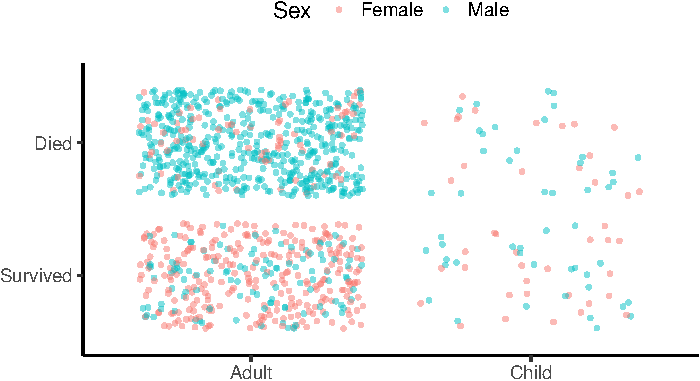
\includegraphics[width=0.8\textwidth]{regression_files/figure-beamer/unnamed-chunk-7-1} \end{center}

\vspace{-5mm}

\footnotesize

Each point represents a person in the data. Color shows whether the
person was male or female. The quadrant in which the point is plotted
shows whether the person was an adult or a child (x-axis) and whether
the person survived or died (y-axis).

\end{frame}

\begin{frame}{Example-- Surviving the Titanic}

Two things we might want to consider are:

\begin{itemize}
\tightlist
\item
  Would the odds ratio for males versus females be different if we
  \textbf{adjusted} for age?
\item
  Is there an \textbf{interaction} between sex and age in the odds of
  death during the sinking of the Titanic?
\end{itemize}

How would you assess these two questions based on a table of the data?

\centering

\begin{tabular}{lllD{.}{.}{0}D{.}{.}{0}}
\toprule
& && \multicolumn{2}{c}{Outcome}\\
\cmidrule{4-4}\cmidrule{5-5}
Sex&Age && \multicolumn{1}{c}{Survived}&\multicolumn{1}{c}{Died}\\
\midrule
Female&Adult  && 267 & 79 \\
      &Child  && 25  & 17 \\
Male  &Adult  && 109 & 500\\
      &Child  && 26  & 23 \\
\bottomrule
\end{tabular}

\end{frame}

\begin{frame}{Adjusting for a variable}

\begin{itemize}
\tightlist
\item
  ``Adjusting'' estimates the association for a predictor and outcome
  while ensuring the comparison is within the same strata of another
  variable (e.g., comparing odds for males versus females while ensuring
  that adults are compared to adults and children to children).
\end{itemize}

\begin{block}{Idea of adjusting for a variable in Titanic example}
We assume there is a constant odds ratio of dying for males versus females, regardless of age. However, in our simple logistic regression, we may not be estimating this odds ratio well because: 
\begin{enumerate}
  \item The proportion of males versus females may differ by age category.
  \item The odds of death may differ by age category.
\end{enumerate}
\end{block}

\end{frame}

\begin{frame}{Adjusting for a variable}

\begin{center}
\includegraphics[width=0.9\textwidth]{images/purity} \end{center}

\vspace{-8mm}

\footnotesize{Figure source: \url{www.xkcd.com}.}

\small

\begin{itemize}
\tightlist
\item
  Adjusting for a variable can help correct for bias from a confounder.
\item
  For continuous outcomes, adjusting for a variable that helps explain
  residual variance in the outcome can improve efficiency
\end{itemize}

\footnotesize{Shisterman et al. (2009) Overadjustment bias and unnecessary adjustment in epidemiologic studies. \textit{Epidemiology} 20(4):488--295.}

\end{frame}

\begin{frame}{Investigating interaction with a variable}

\begin{block}{Idea of interaction in Titanic example}
The odds ratio of dying during the Titanic sinking for males versus females is \textbf{different} within each age category. We will estimate separate odds ratios for adults and children.
\end{block}

\begin{itemize}
\tightlist
\item
  If we find that there is an interaction between sex and age in odds of
  dying, we would say that age \textbf{modifies} the association between
  sex and odds of dying. We would call age an \textbf{effect modifier}
  for this association. (Note that this is \emph{not} mediation!)
\end{itemize}

\end{frame}

\begin{frame}{Example-- Surviving the Titanic}

We can fit a model to estimate the log odds ratio of dying during the
sinking of the Titanic for males versus females, adjusted for age, with
the following regression model:

\[
log(\frac{p_i}{1 - p_i}) = \beta_0 + \beta_1X_{1,i} + \beta_2X_{2,i}
\]

where:

\begin{equation*}
    X_{1,i}=
    \begin{cases}
      0 \text{ if person \textit{i} is female} \\
      1 \text{ if person \textit{i} is male}
    \end{cases}
\end{equation*}

\begin{equation*}
    X_{2,i}=
    \begin{cases}
      0 \text{ if person \textit{i} is an adult} \\
      1 \text{ if person \textit{i} is a child}
    \end{cases}
\end{equation*}

\end{frame}

\begin{frame}{Example-- Surviving the Titanic}

From this logistic regression model, here are the log odds that will be
estimated for each group:

\centering

\begin{tabular}{lcc}
\toprule \\
 & Adult & Child \\
\midrule
Female & $\hat{\beta_0}$ & $\hat{\beta_0} + \hat{\beta_2}$ \\
Male & $\hat{\beta_0} + \hat{\beta_1}$ & $\hat{\beta_0} + \hat{\beta_1} + \hat{\beta_2}$ \\
\bottomrule
\end{tabular}

\vspace{5mm}

\justifying

Notice that these estimates always estimate the same difference in log
odds between males and females within an age category
(\(\hat{\beta_1}\)), regardless of which age category you consider. This
is the estimated log odds ratio for males versus females, \emph{adjusted
for} or \emph{controlling for} age category.

\end{frame}

\begin{frame}{Example-- Surviving the Titanic}

Here are the results from fitting the regression model (``Sex and Age''
column):

\begin{table}
%%%%%%%%%%%%%%%%%%%%%%%%%%%%%%%%%%%%%%%%%%%%%%%%%%%%%%%%%%%%%%%%%%%%%%%%%%%%%%%%%%%%%%%%
%
% Calls:
% Sex only:  glm(formula = Outcome ~ Sex, family = "binomial", data = titanic) 
% Sex and Age:  glm(formula = Outcome ~ Sex + Age, family = "binomial", data = titanic) 
%
%%%%%%%%%%%%%%%%%%%%%%%%%%%%%%%%%%%%%%%%%%%%%%%%%%%%%%%%%%%%%%%%%%%%%%%%%%%%%%%%%%%%%%%%
\begin{tabular}{lD{.}{.}{3}D{.}{.}{3}}
\toprule
&\multicolumn{1}{c}{Sex only}&\multicolumn{1}{c}{Sex and Age}\\
\midrule
(Intercept)&-1.112^{***}&-1.053^{***}\\
&(0.118)&(0.120)\\
Sex: Male/Female&2.467^{***}&2.463^{***}\\
&(0.152)&(0.153)\\
Age: Child/Adult&&-0.641^{*}\\
&&(0.261)\\
\midrule
Log-likelihood&-551.0&-548.0\\
Deviance&1102.0&1096.0\\
AIC&1106.0&1102.0\\
BIC&1115.9&1116.9\\
\bottomrule
\end{tabular}
\end{table}

\end{frame}

\begin{frame}{Example-- Surviving the Titanic}

When we fit our data to the model, we get the following regression
model:

\[
log(\frac{p_i}{1 - p_i}) = -1.0532 + 2.4634X_{1,i} + -0.6413X_{2,i}
\]

where:

\begin{equation*}
    X_{1,i}=
    \begin{cases}
      0 \text{ if person \textit{i} is female} \\
      1 \text{ if person \textit{i} is male}
    \end{cases}
\end{equation*}

\begin{equation*}
    X_{2,i}=
    \begin{cases}
      0 \text{ if person \textit{i} is an adult} \\
      1 \text{ if person \textit{i} is a child}
    \end{cases}
\end{equation*}

\end{frame}

\begin{frame}{Example-- Surviving the Titanic}

Here are the log odds estimated for each group:

\centering

\begin{tabular}{lcc}
\toprule \\
 & Adult & Child \\
\midrule
Female & -1.0532 & -1.0532 - 0.6413 \\
Male   & -1.0532 + 2.4634 & -1.0532 + 2.4634 - 0.6413 \\
\bottomrule
\end{tabular}

\begin{itemize}
\tightlist
\item
  The estimated log odds ratio for males versus females, \emph{adjusted
  for age group}, is \(2.4634\).
\item
  The estimated odds ratio for males versus females, \emph{adjusted for
  age group}, is \(e^{2.4634} = 11.74\).
\item
  The 95\% confidence interval for the log odds ratio is
  \(2.4634 \pm 1.96(0.1527) = (2.164, 2.763)\).
\item
  The 95\% confidence interval for the odds ratio is
  \((e^{2.164}, e^{2.763}) = (8.71, 15.84)\).
\end{itemize}

\end{frame}

\begin{frame}{Example-- Surviving the Titanic}

Here are graphs of the estimated log odds within each group (the dotted
line shows the estimate from the simple logistic regression):

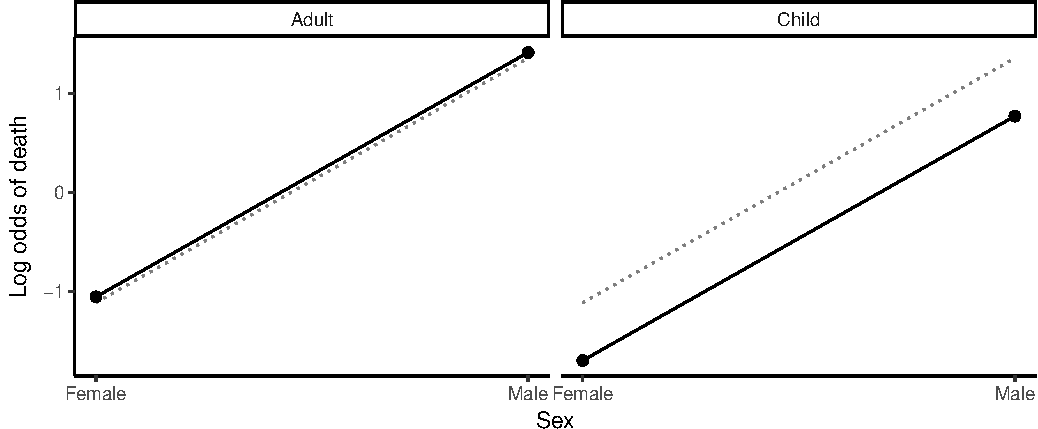
\includegraphics{regression_files/figure-beamer/unnamed-chunk-11-1.pdf}

In this analysis, we made the assumption that the odds ratio for males
versus females is the same within each age category. However, we have
allowed the age categories to have different baseline log odds.

\end{frame}

\begin{frame}{Deviance / Likelihood test statistic}

The deviance and log-likeihood values can be used to calculate test
statistics for hypothesis tests of \textbf{nested} models. Models are
nested if:

\begin{itemize}
\tightlist
\item
  The predictors for one model are a subset of the predictors for the
  other model.
\item
  The models were fit using the same observations.
\end{itemize}

Information criteria (e.g., AIC, BIC) can be used to compare models
whether they are tested or not. However, they can not be used for
specific hypothesis tests.

\end{frame}

\begin{frame}{Example-- Surviving the Titanic}

We can fit a model to estimate the log odds ratio of dying during the
sinking of the Titanic for males versus females, with an interaction for
age, with the following regression model:

\[
log(\frac{p_i}{1 - p_i}) = \beta_0 + \beta_1X_{1,i} + \beta_2X_{2,i} + \beta_3X_{1,i}X_{2,i}
\]

where:

\begin{equation*}
    X_{1,i}=
    \begin{cases}
      0 \text{ if person \textit{i} is female} \\
      1 \text{ if person \textit{i} is male}
    \end{cases}
\end{equation*}

\begin{equation*}
    X_{2,i}=
    \begin{cases}
      0 \text{ if person \textit{i} is an adult} \\
      1 \text{ if person \textit{i} is a child}
    \end{cases}
\end{equation*}

\end{frame}

\begin{frame}{Example-- Surviving the Titanic}

From this logistic regression model, here are the odds that will be
estimated for each group:

\centering

\begin{tabular}{lcc}
\toprule \\
 & Adult & Child \\
\midrule
Female & $\hat{\beta_0}$ & $\hat{\beta_0} + \hat{\beta_2}$ \\
Male & $\hat{\beta_0} + \hat{\beta_1}$ & $\hat{\beta_0} + \hat{\beta_1} + \hat{\beta_2} + \hat{\beta_3}$ \\
\bottomrule
\end{tabular}

\vspace{5mm}

\justifying

Notice that now the difference in log odds for males versus females is
different depending whether the person is an adult (difference in log
odds of \(\hat{\beta_1}\) between males and females) or a child
(difference in log odds of \(\hat{\beta_1} + \hat{\beta_3}\) between
males and females). We are now estimating different odds ratios for
males versus females for the two age categories.

\end{frame}

\begin{frame}{Example-- Surviving the Titanic}

Here are the results from fitting the regression model (``Sex:Age''
column):

\vspace{-5mm}

\begin{table}
\footnotesize
%%%%%%%%%%%%%%%%%%%%%%%%%%%%%%%%%%%%%%%%%%%%%%%%%%%%%%%%%%%%%%%%%%%%%%%%%%%%%%%%%%%%%%%
%
% Calls:
% Sex only:  glm(formula = Outcome ~ Sex, family = "binomial", data = titanic) 
% Sex+Age:  glm(formula = Outcome ~ Sex + Age, family = "binomial", data = titanic) 
% Sex:Age:  glm(formula = Outcome ~ Sex * Age, family = "binomial", data = titanic) 
%
%%%%%%%%%%%%%%%%%%%%%%%%%%%%%%%%%%%%%%%%%%%%%%%%%%%%%%%%%%%%%%%%%%%%%%%%%%%%%%%%%%%%%%%
\begin{tabular}{lD{.}{.}{3}D{.}{.}{3}D{.}{.}{3}}
\toprule
&\multicolumn{1}{c}{Sex only}&\multicolumn{1}{c}{Sex+Age}&\multicolumn{1}{c}{Sex:Age}\\
\midrule
(Intercept)&-1.112^{***}&-1.053^{***}&-1.218^{***}\\
&(0.118)&(0.120)&(0.128)\\
Sex: Male/Female&2.467^{***}&2.463^{***}&2.741^{***}\\
&(0.152)&(0.153)&(0.166)\\
Age: Child/Adult&&-0.641^{*}&0.832^{*}\\
&&(0.261)&(0.339)\\
Sex: Male/Female $\times$ Age: Child/Adult&&&-2.478^{***}\\
&&&(0.456)\\
\midrule
Log-likelihood&-551.0&-548.0&-534.2\\
Deviance&1102.0&1096.0&1068.5\\
AIC&1106.0&1102.0&1076.5\\
BIC&1115.9&1116.9&1096.3\\
\bottomrule
\end{tabular}
\end{table}

\end{frame}

\begin{frame}{Example-- Surviving the Titanic}

When we fit our data to the model, we get the following regression
model:

\[
log(\frac{p_i}{1 - p_i}) = -1.2178 + 2.7411X_{1,i} + 0.8321X_{2,i} + -2.4780X_{1,i}X_{2,i}
\]

where:

\begin{equation*}
    X_{1,i}=
    \begin{cases}
      0 \text{ if person \textit{i} is female} \\
      1 \text{ if person \textit{i} is male}
    \end{cases}
\end{equation*}

\begin{equation*}
    X_{2,i}=
    \begin{cases}
      0 \text{ if person \textit{i} is an adult} \\
      1 \text{ if person \textit{i} is a child}
    \end{cases}
\end{equation*}

\end{frame}

\begin{frame}{Example-- Surviving the Titanic}

Here are the log odds estimated for each group:

\centering

\begin{tabular}{lcc}
\toprule \\
 & Adult & Child \\
\midrule
Female & -1.2178 & -1.2178 + 0.8321 \\
Male   & -1.2178 + 2.7411 & -1.2178 + 2.7411 + 0.8321 - 2.4780 \\
\bottomrule
\end{tabular}

\small

\begin{itemize}
\tightlist
\item
  The estimated log odds ratio for males versus females, \emph{among
  adults}, is \(2.7411\).
\item
  The estimated log odds ratio for males versus females, \emph{among
  children}, is \(2.7411 - 2.4780 = 0.2631\).
\item
  The estimated odds ratio for males versus females is
  \(e^{2.7411} = 15.50\) among adults and \(e^{0.2631} = 1.30\) among
  children.
\item
  The 95\% confidence interval for the log odds ratio among adults is
  \(2.7411 \pm 1.96(0.1661) = (2.416, 3.067)\).
\item
  The 95\% confidence interval for the odds ratio is
  \((e^{2.416}, e^{3.067}) = (11.20, 21.47)\).
\end{itemize}

\end{frame}

\begin{frame}{Example-- Surviving the Titanic}

Here are graphs of the estimated log odds within each group (the dotted
line shows the estimate from the simple logistic regression):

\vspace{-2mm}

\begin{center}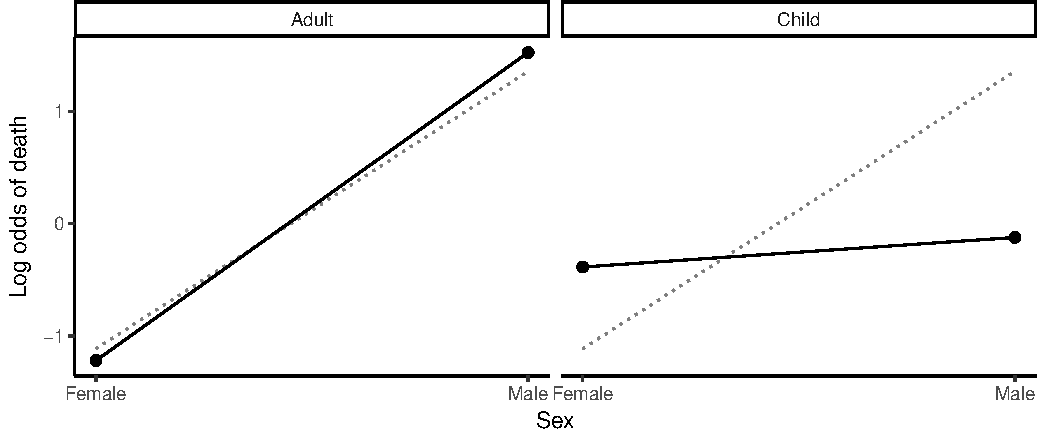
\includegraphics[width=0.9\textwidth]{regression_files/figure-beamer/unnamed-chunk-13-1} \end{center}

\small 

In this analysis, we have estimated \textbf{different} odds ratios
within each age category. These two odds ratios are very different,
indicating evidence of an interation between age and sex on the odds of
dying during the sinking of the Titanic.

\end{frame}

\begin{frame}{Example-- Surviving the Titanic}

\begin{columns}
\begin{column}{0.55\textwidth}
\begin{itemize}
\small
  \item \textbf{Adjusting for age:} The odds ratio for males versus females of dying during the sinking of the Titanic is very similar with or without adjustment for age. 
  \item \textbf{Interaction with age:} There is strong evidence of an interaction between age and sex in the odds of dying during the sinking of the Titanic. While the odds of dying are much higher for males than females among adults, the odds do not vary much by sex among children.
\end{itemize}
\end{column}

\begin{column}{0.45\textwidth}
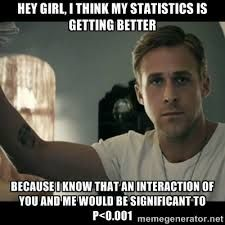
\includegraphics{images/interaction.jpg}
\end{column}
\end{columns}

\end{frame}

\begin{frame}{Example-- Surviving the Titanic}

You could continue expanding the regression model. For example, do you
think that the odds ratio for males versus females should be adjusted
for ticket class? Do you think there might be an interaction between sex
and ticket class? What about age and ticket class?

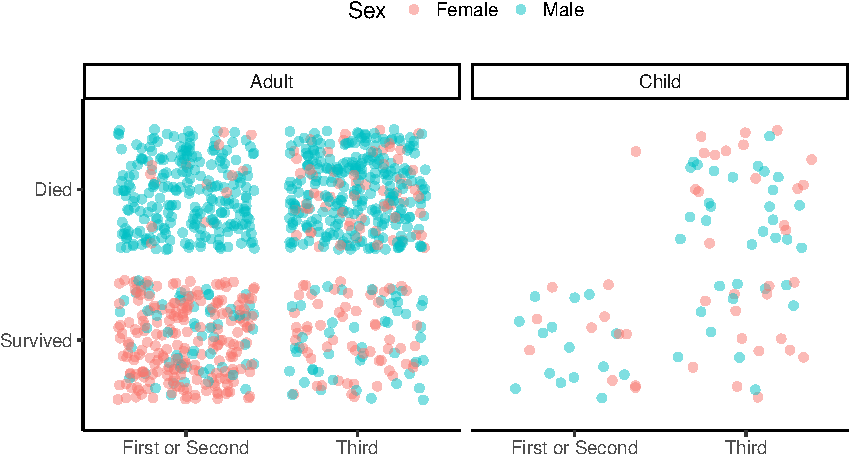
\includegraphics[width=0.85\textwidth]{regression_files/figure-beamer/unnamed-chunk-14-1}

\end{frame}

\begin{frame}{Generalized linear models}

Different forms of GLMs are distinguished by (1) the link function and
(2) the distribution of the outcome.

\centering \small

\begin{tabular}{lccc}
\toprule \\
 & Example & & Outcome \\
Model & outcome & Link &  distribution \\
\midrule
Linear & Continuous & Identity: $E(Y)$ & Normal\\
Logistic & Binary & Logit: $log(\frac{E(Y)}{1-E(Y)})$ & Binomial\\
Poisson & Count & Log: $log(E(Y))$ & Poisson \\
Log-binomial & Binary & Log: $log(E(Y))$ & Binomial\\
Additive risk & Binary & Identity: $E(Y)$  & Binomial\\
\bottomrule
\end{tabular}

\end{frame}

\begin{frame}{Generalized linear models-- link functions}

Here are how the systematic part of a GLM looks for different link
functions:

\begin{block}{Identity link:}
$$
E([Y_i]) = \beta_0 + \beta_1X_1 + \beta_2X_2 + ...
$$
\end{block}

\begin{block}{Log link:} 
$$
log(E[Y_i]) = \beta_0 + \beta_1X_1 + \beta_2X_2 + ...
$$
\end{block}

\begin{block}{Logit link:}
$$
log\left(\frac{E[Y_i]}{1 - E[Y_i]}\right) = \beta_0 + \beta_1X_1 + \beta_2X_2 + ...
$$
\end{block}

\end{frame}

\begin{frame}{Survival analysis}

What if we were interested in how long people survived instead of
whether they survived?

\vspace*{-5mm}

\begin{center}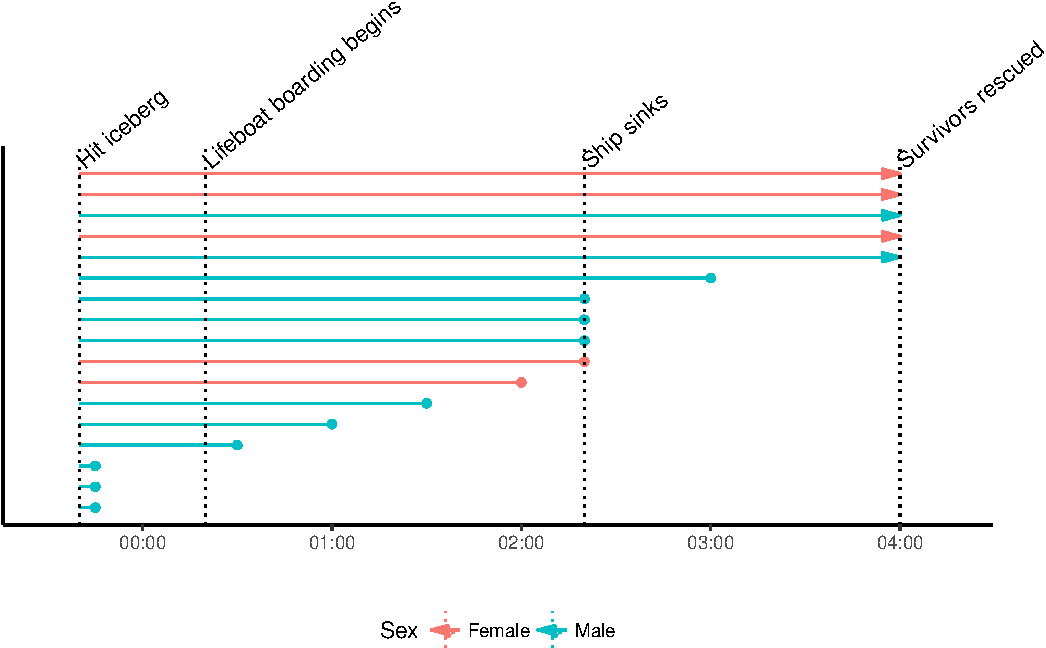
\includegraphics[width=0.85\textwidth]{regression_files/figure-beamer/unnamed-chunk-15-1} \end{center}

\vspace*{-5mm}

\footnotesize
Each line shows a person on the Titanic. The lines with arrows are
people who survived. The lines with points show people who died, with
the point at the time they died.

\end{frame}

\begin{frame}{Survival analysis}

\begin{columns}
\begin{column}{0.5\textwidth}
Characteristics of survival analysis:
\begin{itemize}
  \item Outcome is no longer binary (survived / died)
  \item Outcome is survival time (time to event)
  \item Right-censored data-- time to event is longer than follow-up time and so unobserved
\end{itemize}
\end{column}

\begin{column}{0.5\textwidth}
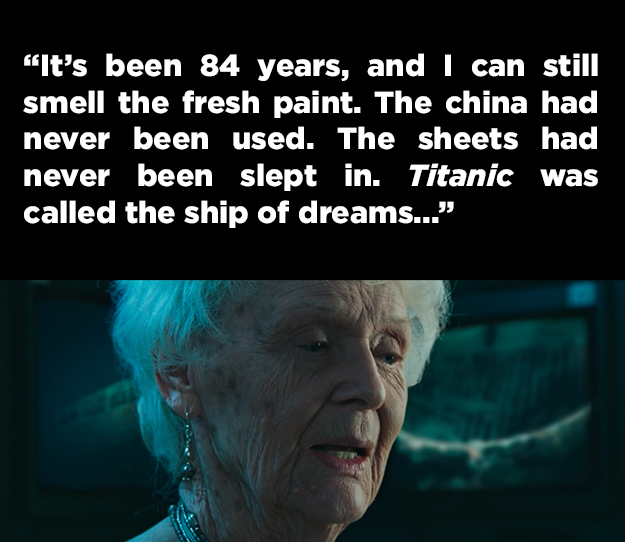
\includegraphics{images/survival_analysis.png}
\end{column}
\end{columns}

\end{frame}

\begin{frame}{Survival analysis}

For a survival analysis, you can model the log hazard ratio as a linear
function of predictors using a proportional hazard model:

\[
log[HR(\mathbf{x_i})] = log\frac{h(t|\mathbf{x_i})}{h_0(t)} = \beta_1X_{1,i} + \beta_2X_{2,i} + ... 
\]

where:

\begin{itemize}
\tightlist
\item
  \(h_0(t)\): The baseline hazard at time \emph{t}
\item
  \(h(t|\mathbf{x_i})\): The hazard at time \emph{t} given
  characteristics \(\mathbf{x_i}\)
\item
  \(HR(\mathbf{x_i})\): The hazard ratio for person \emph{i}
\end{itemize}

This model assumes \emph{proportional hazards}. Cox proportional hazard
model is a popular semi-parameteric model to fit.

\end{frame}

\begin{frame}{Survival analysis}

In the Titanic example, if we were interested in how survival time is
associated with sex, we could fit the following Cox proportional hazards
model:

\[
log[HR(\mathbf{x_i})] = log\frac{h(t|X_{1,i})}{h_0(t)} = \beta_1X_i 
\]

where:

\[
    X_i=
    \begin{cases}
      0 \text{ if person i is female} \\
      1 \text{ if person i is male}
    \end{cases}
\]

\end{frame}

\begin{frame}{Association versus causation}

An important caveat of all these models is that all they guarantee to
estimate is association, not causation. There are ways to use regression
modeling as a tool in causal inference, but using a regression model
does not guarantee a causal interpretation.

\centering

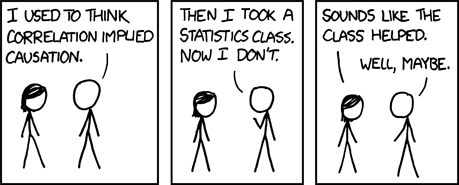
\includegraphics[width = 0.8\textwidth]{images/correlation.png}

\justifying

\footnotesize{Source: \url{www.xkcd.com}}

\end{frame}

\begin{frame}{Multicollinearity}

\begin{columns}
\begin{column}{0.5\textwidth}
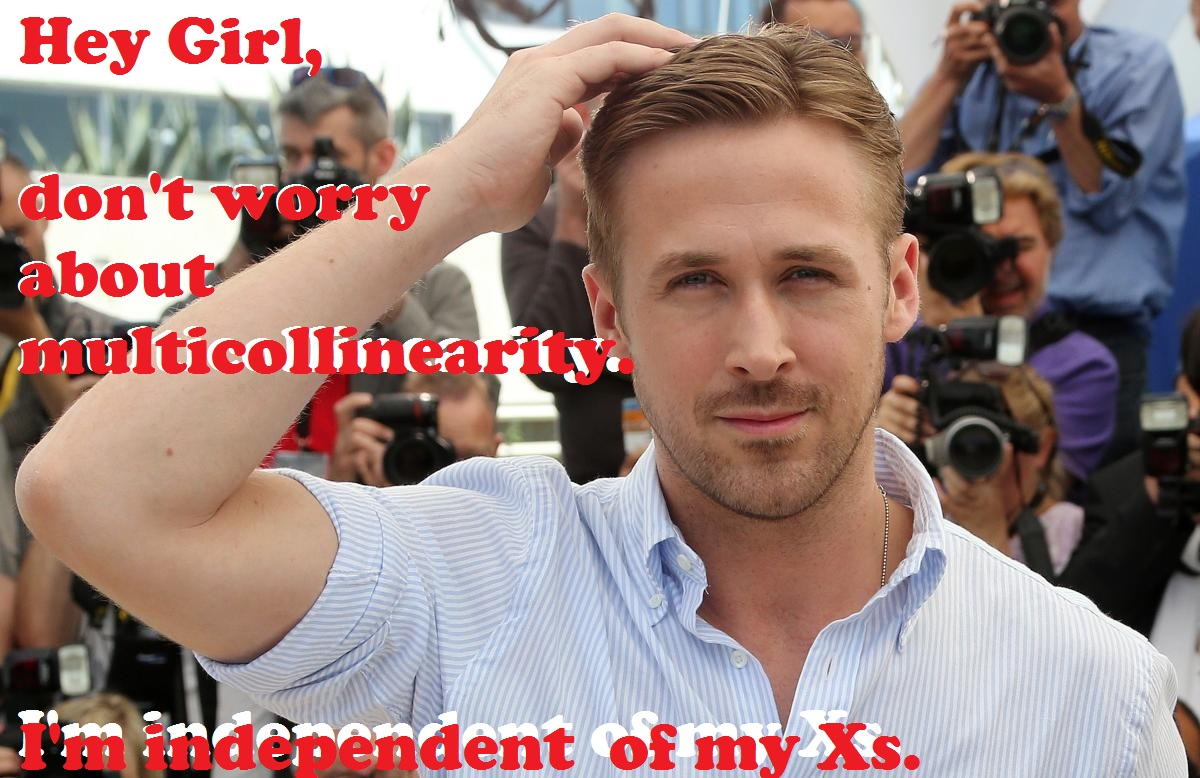
\includegraphics{images/multicollinearity.jpg}
\end{column}

\begin{column}{0.5\textwidth}
A second caveat is that you need to careful of including multiple predictors that are strongly correlated. If not, you will run into problems from \textbf{multicollinearity}-- the regression model will struggle to separate estimated coefficients between the correlated variables.
\end{column}
\end{columns}

\begin{itemize}
\tightlist
\item
  For the Titanic example, a model that included ticket class and ticket
  price might suffer from multicollinearity.
\item
  Implications: (1) instability of coefficient estimates and (2) large
  standard errors for coefficient estimates.
\end{itemize}

\end{frame}

\begin{frame}{Model assumptions}

\begin{columns}
\begin{column}{0.5\textwidth}
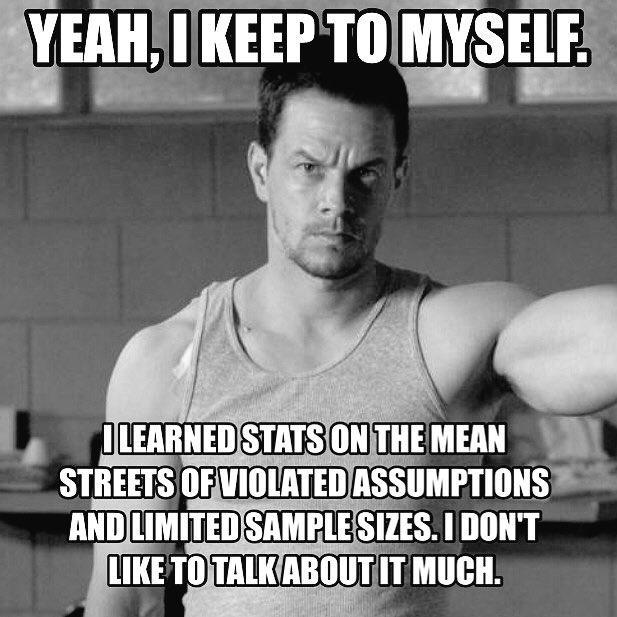
\includegraphics{images/violated_assumptions.jpg}
\end{column}

\begin{column}{0.5\textwidth}
Assumptions of GLMs: 
\begin{itemize}
  \item Independence assumption (observations are independently distributed)
  \item Outcome follows the specified distribution for a fixed set of covariates
  \item For continuous predictors, relationship with $g(E[Y_i])$ is linear
\end{itemize}
\end{column}
\end{columns}

\end{frame}

\begin{frame}{Non-independent outcomes}

\begin{columns}
\begin{column}{0.54\textwidth}
\small
In epidemiological studies, the independence assumption is often violated. Examples of when the independence assumption might be violated include:
\begin{itemize}
  \item Repeated measures / longitudinal data
  \item Hierarchical / clustered data (families, schools, multi-site clinical trials)
\end{itemize}
In the Titanic example, the independence assumption might be violated because many of the passengers were traveling as families, and survival outcomes might be more similar within families than between families.
\end{column}

\begin{column}{0.45\textwidth}
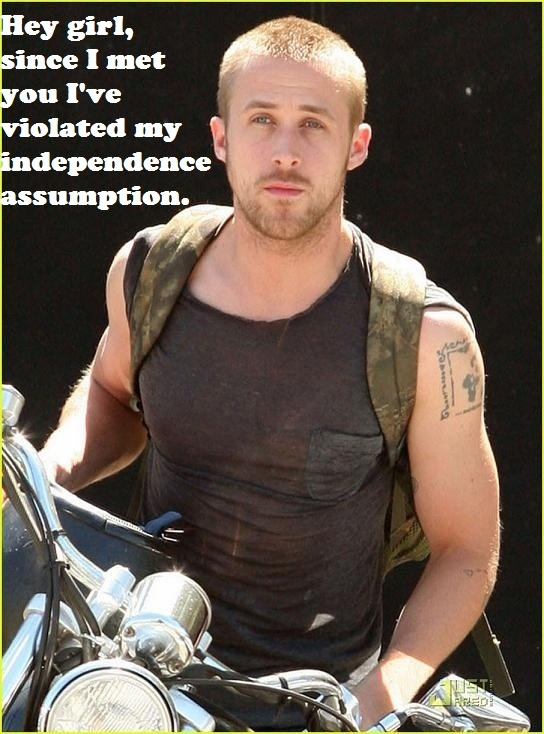
\includegraphics[width = 0.9\textwidth]{images/independence_assumption.jpg}
\end{column}
\end{columns}

\end{frame}

\begin{frame}{Non-independent outcomes}

\begin{columns}
\begin{column}{0.5\textwidth}
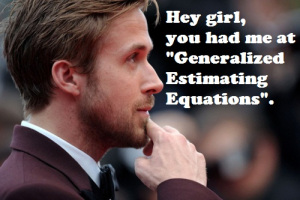
\includegraphics{images/GEE.jpg}
\end{column}

\begin{column}{0.5\textwidth}
There are a number of ways to model data in which the independence assumption is violated. A popular one in epidemiological studies are \textbf{Generalized Estimating Equations} (GEEs).
\end{column}
\end{columns}

\begin{itemize}
\tightlist
\item
  GEEs accomodate correlated observations.
\item
  You must specify which variables indicate clustering (e.g., family in
  the Titanic example).
\item
  You must also specify a ``working correlation structure'' (e.g.,
  exchangeable correlation structure; autoregressive correlation
  structure).
\end{itemize}

\end{frame}

\begin{frame}{Non-independent outcomes}

For more on GEEs in epidemiologic studies:

\begin{itemize}
\tightlist
\item
  Hanley et al. (2003) Statistical analysis of correlated data using
  generalized estimating equations: an orientation.
  \textit{American Journal of Epidemiology.}
\item
  Hubbard et al. (2009) To GEE or not to GEE: comparing estimating
  function and likelihood-based methods for estimating the associations
  between neighborhoods and health. \textit{Epidemiology}.
\end{itemize}

\end{frame}

\end{document}
